% !TEX root = ../notes_template.tex

\chapter{복소수와 기하학적 의미}


이 장에서는 복소해석학을 펼칠 무대를 만들기 위해
다음 3가지 중심 주제를 다룬다.

\begin{itemize}
\item[(1)] 복소수의 집합과 연산을 정의하고 실수체의 확장으로서 복소수체 $\mathbb C$를 만든다.
\item[(2)] $\mathbb C$의 원소는 평면 $\mathbb R^2$위의 점으로 표시할 수 있으며, 복소수체 $\mathbb C$의 연산에 대하여
기하학적 의미를 부여할 수 있다. 복소수체와 평면위의 점의 대응 관계로부터
$\mathbb C$에 평면의 유클리드 위상을 가져올 수 있다.
\item[(3)] 끝으로 복소해석학의 기초함수인 지수함수를 공부한다.
또한, 지수함수와 관련된 기본함수인 삼각함수와 로그함수도 살펴본다. 
\end{itemize}

\section{복소수체}

{\bf 복소수}는 실수의 순서쌍으로 정의한다. 예를 들면,
$$
(1,0), \ (0,1), \ (0,0), \ \left(-\dfrac34, \sqrt{2} \right)
$$
는 모두 복소수로 간주할 수 있다.
복소수 전체의 집합 $\mathbb R \times \mathbb R$을 $\mathbb C$라 표기한다. 즉,
$$
\mathbb C = \left\{ z = (x,y) \,:\, x\in \mathbb R, \text{ 이고 } y\in \mathbb R \right\}.
$$

복소수 $z=(x,y)\in \mathbb C$ ($x,y \in \mathbb R$)에 대하여
실수 $x$는 $z$의 실수부, $y$는 $z$의 허수부라고 한다.

집합 $\mathbb C$의
복소수 $(x_1, y_1)$, $(x_2, y_2)$에 대하여
덧셈 ``$+$''과 곱셈 ``$\cdot$''을 다음과 같이 정의한다.
\begin{gather*}
(x_1, y_1) + (x_2, y_2) = (x_1+x_2, y_1+y_2), \\
(x_1, y_1) \cdot (x_2, y_2) = (x_1x_2 - y_1y_2, x_1y_2 + x_2y_1).
\end{gather*}
이 연산에 따라 $\mathbb C$는 체(field)가 된다. 즉,
\begin{itemize}
\item[(F1)]  $(\mathbb C, +)$는 가환군(Abelian group)이다.
\item[(F2)] $(\mathbb C\setminus \{0\}, \cdot)$는 가환군이다.
\item[(F3)] $a,b,c\in\mathbb C$에 대하여 분배법칙이 성립한다:  $(a+b)\cdot c = a\cdot c + b\cdot c$.
\end{itemize}

(F1)에서 가환군이란
연산 $+$에 대하여 결합법칙, 교환법칙이 성립하며,
모든 $(x,y)$에 대하여
$$
(x,y) + (0,0) = (x,y) = (0,0) + (x,y)
$$
를 만족하는 
항등원 $(0,0)$과 
$$
(x,y) + (-x,-y) = (0,0) = (-x,-y) + (x,y)
$$
를 만족하는 덧셈의 역원 $(-x, -y)$이  존재한다는 뜻이다.

유사하게, (F2)에서 곱셈의 항등원 $(1,0)$이 존재하고, 복소수 $(x,y) \in \mathbb C \setminus\{0,0\}$의
곱셈의 역원은 다음과 같다.
\begin{equation} \label{eq:1.1}
\left( \dfrac{x}{x^2+y^2}, \dfrac{-y}{x^2+y^2} \right).
\end{equation}

\begin{salt_exercise}
식 \eqref{eq:1.1}\이 복소수 $(x,y) \in \mathbb C \setminus\{0,0\}$의 곱셈의 역원이 됨을 직접 확인하라.
\end{salt_exercise}


\begin{salt_prop}
$(\mathbb C, +, \cdot)$는 체(field)이다.
\end{salt_prop}

실수  $\mathbb R$은 복소수 $\mathbb C$에 ``포함된다''.
실제로, 복소수 $\mathbb C$안에 $\mathbb R$을 넣어
실수 $\mathbb R$을 $\mathbb C$의 부분체(subfield)로 볼 수 있다.
$$
x \mapsto (x,0)
$$
을 이용하여 실수 $x$를 복소수 $(x,0)$로 보내는 대응 규칙은
단사인 체의 준동형사상(field homomorphism)이다.
즉, 덧셈과 곱셈이 보존되며 서로 다른 실수는 다른 복소수에 대응시키는 사상이다.

\begin{center}
\begin{tabular}{|ccc|} \hline
$\mathbb R$ & & $\mathbb C$ \\ \hline \hline
$x$ & $\mapsto$ & $(x,0)$ \\ 
$x_1+x_2$ & $\mapsto$ & $(x_1+x_2,0) = (x_1,0) + (x_2,0)$ \\ 
$x_1\cdot x_2$ & $\mapsto$ & $(x_1\cdot x_2,0) = (x_1,0) \cdot (x_2,0)$ \\ 
$1$ & $\mapsto$ & $(1,0)$ \\
$0$ & $\mapsto$ & $(0,0)$ \\
\hline
\end{tabular}
\end{center}

따라서 이 사상을 이용한 동일화에 따라 모든 실수는 복소수로 볼 수 있다.
예를 들어 실수 $\sqrt{2}$는 복소수 $(\sqrt{2},0)$로 볼 수 있다.
이런 생각에 익숙하지 않을 수도 있겠으나 우리는 이미 초등학교 과정에서
비슷한 동일화를 경험한 적이 있다. 정수를 유리수의 일부로 동질화하는
다음 예를 보자.
$$
\mathbb Z  \ni 3 = \frac31 \in \mathbb Q
$$
이를 이해하려고 밤잠을 설친 적은 없지 않은가!

실수 해 $x\in\mathbb R$를 갖지 않는 방정식
$$
x^2+1=0
$$
을 복소수 밤위에서 다루면 해를 구할 수 있다.
$$
(0,1)\cdot (0,1) + (1,0) = (-1,0) + (1,0) = (0,0).
$$
$(0,1)$을 나타내는 특별한 기호로 $i$를 도입하면 이 방정식을 다음과 같이 쓸 수 있다.
$$
i^2+1=0,
$$
여기서 실수 $1$과 $0$은 각각 복소수 $(1,0)$과 $(0,0)$에 대응된다.

이제부터 실수  $x,y$로 만든 복소수 $(x,y)$를 $x+yi$로 쓰자.
$$
(x,y) = \underbrace{(x,0)}_{\equiv x} +  \underbrace{(y,0)}_{\equiv y}
\cdot  \underbrace{(0,1)}_{\equiv i} = x+yi.
$$
복소수 곱셈은 교환법식이 성립하고, 특히 $yi = iy$이므로,
$x+yi = x+iy$이다.

\begin{salt_exercise} %1.2
$\theta \in \left(-\dfrac{\pi}2, \dfrac\pi2 \right)$에 대하여
$\dfrac{1+i\tan\theta}{1-i\tan\theta}$를 $x+yi$ 꼴로 표시하면?
\end{salt_exercise}

{\bf 복소수 발견의 역사: }
대중적인 믿음과는 달리 역사적으로 수학자들이 복소수를 진지하게 받아들이게 된 것은 
2차 방정식이 아니라 3차 방정식을 풀 필요가 있었기 때문이다. 요지는 다음과 같다.
16세기 경 포물선 $y=x^2$과 직선 $y=-bx-c$의 교점을 구하는  방법으로 
 방정식
$$
ax^2 + bx + c = 0
$$
을 풀려는 시도가 있었다. 
이러한 기하학적 해석에 근거하여,
포물선  $y=x^2$ 이 직선 $y=-1$과 만나지 않으므로
실계수 2차방정식 $x^2+1=0$이 실수해를 갖지 않음을 쉽게 알 수 있었다.
%%%%%%
그림 \ref{fig-1-1}의 왼쪽 그래프를 참고하라.

\begin{figure}[!h]
\begin{center}
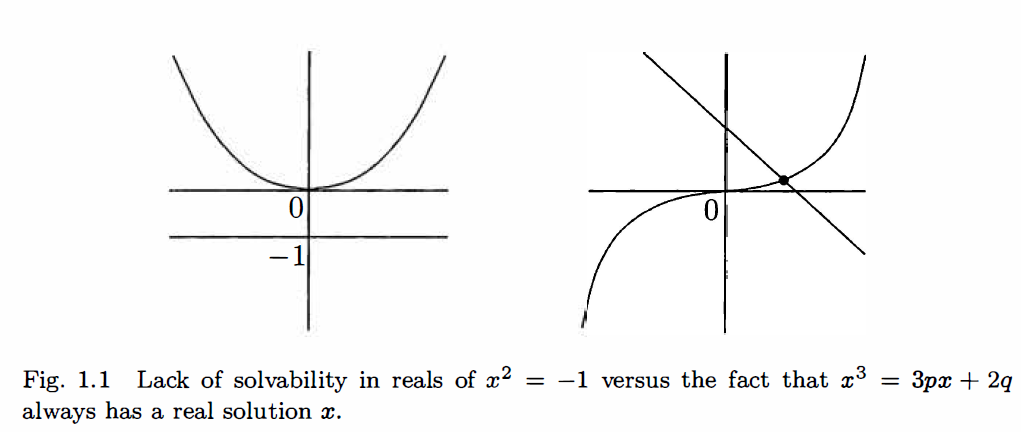
\includegraphics[width=0.6\textwidth]{./SaltChapter/fig-1-1}
\end{center}
\caption{실근이 존재하지 않는 방정식 $x^2=-1$과 항상 실근을 갖는 $x^3=3px+2q$}
\label{fig-1-1}
\end{figure}

Cardano (1501-1576)는 3차방정식 $x^3=3px+2q$의 실근을 구하는 다음 공식을 만들었다.
$$
x = \sqrt[3]{q+ \sqrt{q^2-p^3}} + \sqrt[3]{q- \sqrt{q^2-p^3}}
$$
예를 들어, $p=2$, $q=3$일 때 방정식 $x^3=6x+6$은 $x=\sqrt[3]{4}+\sqrt[3]{2}$를 해로 가진다.
한편, 중간값 정리에 의해 3차함수 $y=x^3$은  항상 $y=3px+2q$와 만난다.
그림 \ref{fig-1-1}의 오른쪽 그래프를 참고하라.
하지만 $p=5$, $q=2$로 방정식 $x^3=15 x+4$을 만들면 $q^2-p^3= -121<0$이 되어
실수만으로는 Cardano의 공식을 적용하지 못한다.
그럼에도 불구하고 우리는 $x=4$가 실근이 됨을 확인할 수 있다.
$$
4^3 = 64 = 60 + 4 = 15\cdot 4 + 4.
$$
Cardano 공식이 나온지 30년 후, Bombelli가 복소수 연산을 도입하면
Cardano 공식으로 원하는 실근을 도출할 수 있음을 제안하였다.
다음 등식이 성립할 수 있을까?
$$
x = \sqrt[3]{2+11i} + \sqrt[3]{2-11i} \stackrel{?}{=} 4.
$$
$(2+i)^3 = 2+11i$이고 $(2-i)^3 = 1-11i$임을 이용하면
세제곱근 값으로부터 위 등식이 성립함을 알 수 있다.
따라서 Bombelli의 결과로부터 실수 문제에도 복소수 연산이 연결될 수 있음이 입증되었다.
그때부터 복소수가 수학의 주류에 들어가게 되었다.

\begin{salt_exercise} \label{ex-1-3}
양의 부분집합 $P\subset \mathbb F$가 있어 다음을 만족하면
체 $\mathbb F$는 순서(ordered)를 갖는다고 한다.
\begin{itemize}
\item[(P1)] 모든 $x,y\in P$에 대하여, $x+y\in P$.
\item[(P2)] 모든 $x,y\in P$에 대하여, $x\cdot y \in P$
\item[(P3)] 모든 $x\in P$에 대하여, 다음 3가지 중  정확히 한가지만 참이다.
$$
1^{\circ} \ x=0. \quad 2^{\circ} \ x\in P. \quad 3^{\circ} \ -x\in P.
$$
\end{itemize}
예를 들면, $P:=(0,\infty)$를 양의 부분집합이라 하면
실수체 $\mathbb R$은 순서를 갖는다.
( 순서를 갖는 체 $\mathbb F$에서 두 원소 $x,y\in \mathbb F$의 관계 $>_P$를
$y>_P x$는 $y-x \in P$로 정의하여 대소관계를 정할 수 있다.)
복소수 $\mathbb C$는 순서를 가질 수 없음을 보여라. \\[1ex]
힌트: $x:=i$에 대하여 $x\cdot x$를 살펴보라.
\end{salt_exercise}

\section{복소수의 기하학적 표현}

$\mathbb C = \mathbb R^2$이므로, 
그림 \ref{fig-1-2}와 같이 복소수를 평면위의 점에 대응시킬 수 있다.

\begin{figure}[!h]
\begin{center}
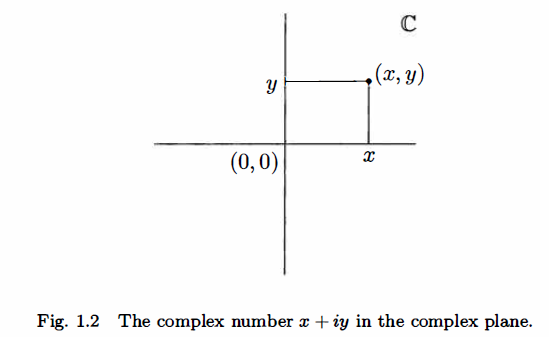
\includegraphics[width=0.5\textwidth]{./SaltChapter/fig-1-2}
\end{center}
\caption{복소평면에 표시한 복소수 $x+iy$}
\label{fig-1-2}
\end{figure}

복소평면은 Argrand\footnote{ 
Jean-Robert Argand (1768-1822)의 이름에서 따온 것이다.
Caspar Wessel (1745-1818)이 더 먼저 사용하긴 했으나.}
평면이라고도 불린다.

\begin{salt_exercise} \label{ex-1-4}
다음 복소수를 복소평면 위의 점으로 표시하라.
$$
0, \quad 1 , \quad -\frac32, \quad i, \quad -\sqrt{2}i,
\quad \cos \frac\pi3 + i\sin\frac\pi3.
$$
\end{salt_exercise}

따라서 복소수 $\mathbb C$는 {\bf 집합}으로서 평면 $\mathbb R^2$로 간주할 수 있다.
$\mathbb C$에 정의된 체의 연산이 평면에서 기하학적 의미를 가질까?
우리는 앞으로 실제로 의미가 있음을 살펴볼 것이다.
$\mathbb C$의 덧셈은 평면벡터의 덧셈이고
곱셈은 조금 더 특별한 의미를 갖는다.

{\bf 복소수 덧셈의 기하학적 의미: }
복소수를 평면 위의 점으로 간주하고 복소수의 덧셈을 $\mathbb R^2$의 벡터 합으로 
정의하는 것이 자연스럽다. 
벡터 합은 두 벡터를 결합하는 일반적인 방식으로 정의한다.
즉, $(0,0)$과 두 복소수를 잇는 선분으로 이루어진 평생사변형을 완성시킬 때
$(0,0)$과 대각선의 반대에 있는 점을 두 복소수의 합이 된다.
그림 \ref{fig-1-3}\을 참고하라.

\begin{figure}[!h]
\begin{center}
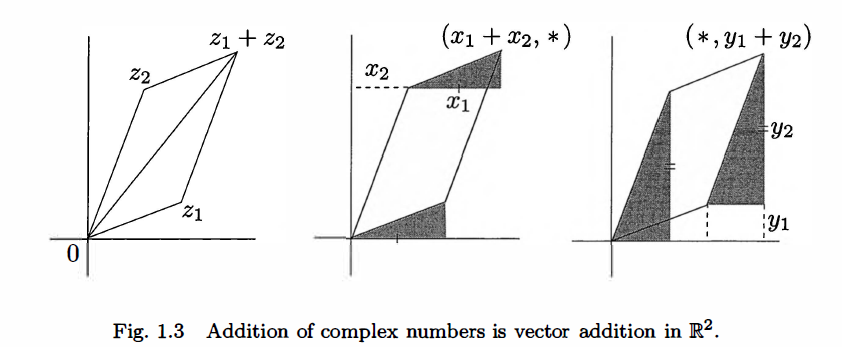
\includegraphics[width=0.8\textwidth]{./SaltChapter/fig-1-3}
\end{center}
\caption{복소수 덧셈은 $\mathbb R^2$의 벡터 합이다.}
\label{fig-1-3}
\end{figure}

{\bf  복소수 곱셈의 기하학적 의미: }
이제 복소수 곱셈이 가진 특별한 기하학적 의미를 살펴보자.
이를 위해 편의상 극좌표를 사용한다.
$(x,y)\in\mathbb R^2$이 극좌표 $r\ge 0$와 $\theta\in(-\pi,\pi]$로 표현된다고 하자.
이는 원점에서 $(x,y)$까지의 거리를 $r(\ge0)$이고,
$(0,0)$에서 $(x,y)$를 잇는 반직선이 $x$-축의 양의 방향과 이루는 각이 $\theta$가 된다는 뜻이다.
($(x,y)$가 원점 $(0,0)$인 경우, $\theta=0$으로 정한다.)

\begin{figure}[!h]
\begin{center}
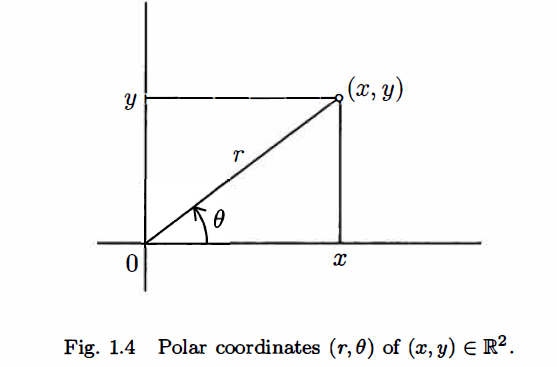
\includegraphics[width=0.5\textwidth]{./SaltChapter/fig-1-4}
\end{center}
\caption{복소수 $(x,y)\in\mathbb R^2$의 극좌표 표현 $(r, \theta)$}
\label{fig-1-4}
\end{figure}

그림 \ref{fig-1-4}의 직각삼각형으로부터 다음 관계를 얻는다.
\begin{gather*}
x = r \cos\theta, \\
y = r \sin \theta.
\end{gather*}
이로부터 복소수를 극좌표 $(r,\theta)$로 표현할 수 있다.
$$
x + yi = r\cos\theta +(r\sin \theta)i
= r(\cos\theta + i\sin \theta).
$$
이제 복소수 곱셈의 기하학적으로 해석하자.
두 복소수를 모두 극좌표로 쓰면
\begin{gather*}
z_1 = r_1 (\cos\theta_1 + i\sin\theta_1), \\
z_2 = r_2 (\cos\theta_2 + i\sin\theta_2),
\end{gather*}
삼각함수의 덧셈정리로부터 다음을 얻는다.
\begin{align*}
z_1\cdot z_2 &= r_1(\cos\theta_1+i\sin\theta_1) \cdot r_2(\cos\theta_2+i\sin\theta_2) \\
&= r_1r_2 (\cos\theta_1\cos\theta_2 - \sin\theta_1\sin\theta_2 +
i(\cos\theta_1\sin\theta_2 + \cos\theta_2\sin\theta_1)) \\
&= r_1r_2(\cos(\theta_1 +\theta_2) + i \sin(\theta_1 +\theta_2)).
\end{align*}
따라서 $z_1\cdot z_2$는 극좌표로 $(r_1r_2, \theta_1+\theta_2)$이다.
다시 말하면, 
$z_1\cdot z_2$의 편각은
$z_1$과 $z_2$가 각각 실수축의 양의 방향과 이루는 각을 더하여 얻을 수 있고,
원점에서의 거리는 각각의 거리를 곱하여 얻는다.
그림 \ref{fig-1-5}\를 참고하라.

\begin{figure}[!h]
\begin{center}
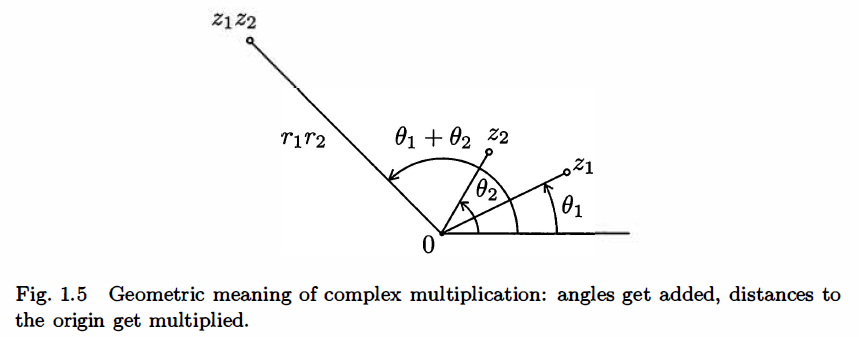
\includegraphics[width=0.5\textwidth]{./SaltChapter/fig-1-5}
\end{center}
\caption{복소수 곱셈의 기하학적 의미: 각은 더하고, 원점에서의 거리는 곱한다.}
\label{fig-1-5}
\end{figure}

특별한 경우로 원점에서의 거리가 $1$인 복소수
$\cos\alpha + i \sin\alpha$를 곱하는 경우를 생각해보자.
그러면 위의 식으로부터 $z\in\mathbb C$와의 곱
$z\cdot(\cos\alpha + i\sin\alpha)$는 
원점과 $z$를 연결하는 직선을 반시계방향으로 $\alpha$만큼 회전시켜 얻을 수 있다.
특히, $z$에 
$$
i = 0 + i\cdot 1 = \cos\frac\pi2 + i \sin\frac\pi2
$$
를 곱하면 반시계방향으로 $90^{\circ}$ 회전한 결과를 얻는다.

\begin{figure}[!h]
\begin{center}
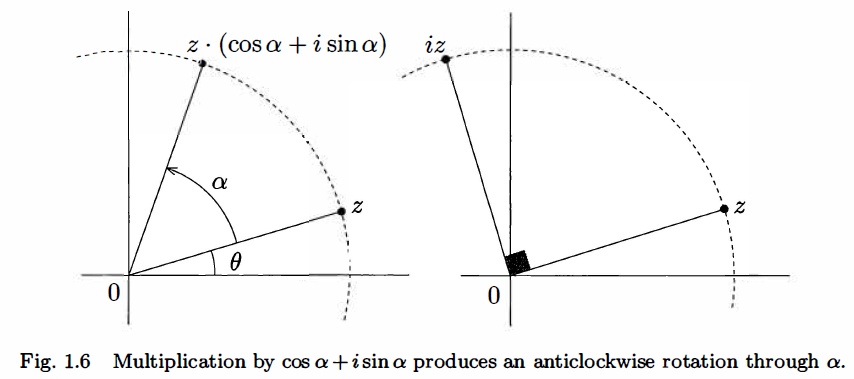
\includegraphics[width=0.8\textwidth]{./SaltChapter/fig-1-6}
\end{center}
\caption{$\cos\alpha + i \sin\alpha$를 곱하면 반시계방향으로 $\alpha$만큼 회전한 결과를 얻는다.}
\label{fig-1-6}
\end{figure}

{\bf 드 므와브르(De Moivre) 정리와 $n$차 제곱근 :}
모든 자연수 $n\in\mathbb N$에 대하여
$$
(\cos\theta + i\sin\theta)^n = \cos(n\theta) + i\sin(n\theta)
$$
가 성립하며 이를 드 므와브르 정리라 한다.

\begin{salt_exercise} \label{ex-1-5}
드 므와브르의 정리를 이용하여
삼각함수의 3배각 공식 $\cos (3\theta) = 4(\cos\theta)^3 - 3\cos\theta$을 증명하라.
\end{salt_exercise}

\begin{salt_exercise} \label{ex-1-6}
$(1+i)^{10}$을 직접 전개하지 않고 $x+iy$ ($x,y$는 실수)의 꼴로 써라?
삼각함수의 3배각 공식 $\cos (3\theta) = 4(\cos\theta)^3 - 3\cos\theta$을 증명하라.
\end{salt_exercise}

\begin{salt_exercise} \label{ex-1-7}
$(2+i)(3+i)$를 이용하여
$\dfrac\pi4 = \tan^{-1}\dfrac12 + \tan^{-1}\dfrac13$을 증명하다.
\end{salt_exercise}

\begin{salt_exercise} \label{ex-1-8}
가우스 정수(Gaussian integer)는 
$m, n$이 정수일 때, $m+in$꼴의 복소수로
복소평면 위의 정수 격자점을 이룬다.
모든 꼭지점이 가우스 정수가 되도록 정삼각형을 그리는 것을 불가능함을 증명하라. \\[1ex]
힌트: 한변의 회전으로 다른 변을 만들 수 있고, $\sqrt{3}\not\in \mathbb Q$임을 이용하라.
\end{salt_exercise}

드 므와브르 공식을 이용하면
복소수  $z$의 $n$ 제곱근
즉, $w^n=z$를 만족하는 복소수 $w$를 쉽게 구할 수 있다.
우선 적당한 $r\ge0$과 $\theta\in[0,2\pi)$에 대하여 $z=r(\cos\theta + i \sin\theta)$로 쓰자.
$w= \rho(\cos\alpha + i\sin\alpha)$가 $w^n=z$를 만족한다면,
$$
w^n = \rho^n\left( \cos(n\alpha) + i\sin(n\alpha)\right) = r(\cos\theta + i\sin\theta)= z.
$$
양변은 원점에서의 거리가 같으므로 $\rho^n=r$을 얻는다.
$\rho$와 $r$이 음수가 아니므로 $\rho = \sqrt[n]{r}$이다.
한편 $w^n$이 실수축의 양의 방향과 이루는 각 $n\alpha$는 
집합 $ \{ \ldots, \theta - 4\pi, \theta - 2\pi, \theta, \theta+2\pi, \theta+4\pi, \ldots\} $에 속한다.
$0$이 아닌 $z$가 실수축의 양의 방향과 이루는 각은 $2\pi$의 정수배 차이를 무시하면 유일하게 결정되므로
$\theta$ 대신 $\theta + 2\pi k$ ($k$는 정수)로도 쓴다. 그림 \ref{fig-1-7}\을 참고하라.

\begin{figure}[!h]
\begin{center}
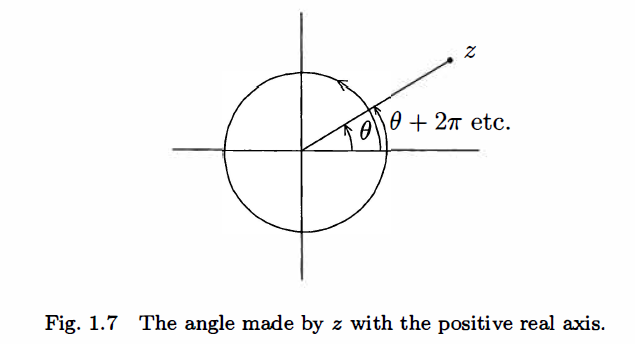
\includegraphics[width=0.7\textwidth]{./SaltChapter/fig-1-7}
\end{center}
\caption{복소수 $z$가 실수축의 양의 방향과 이루는 각}
\label{fig-1-7}
\end{figure}

이제 $\alpha \in \left\{ \dfrac{\theta}{n}+ \dfrac{2\pi}{n}k \,:\, k\in\mathbb Z \right\}$로부터
서로 다른 $w$가 되는 $\alpha$만 쓰면 다음과 같다.
$$
\alpha \in \left\{
\dfrac\theta n,  \dfrac\theta n+ \dfrac{2\pi}n, \dfrac\theta n + 2\cdot \dfrac{2\pi}n, \ldots,
\dfrac\theta n+ (n-1)\cdot \dfrac{2\pi}n
\right\}.
$$
특히, $z=1$일 때, $1$의 $n$제곱근은 원에 내접하는 정$n$각형의 꼭지점이다.
그림 \ref{fig-1-8}을 보라.
\begin{figure}[!h]
\begin{center}
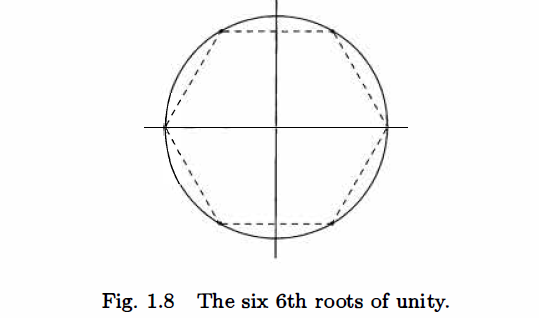
\includegraphics[width=0.7\textwidth]{./SaltChapter/fig-1-8}
\end{center}
\caption{$1$의 $6$ 제곱근 $6$개}
\label{fig-1-8}
\end{figure}

\begin{salt_exercise} \label{ex-1-9}
$w^4=-1$을 만족하는 모든 복소수 $w$를 찾아
복소평면에 표시하라.
\end{salt_exercise}

\begin{salt_exercise} \label{ex-1-10}
$z^6-z^3-2=0$을 만족하는 모든 복소수 $z$를 구하라.
\end{salt_exercise}

\begin{salt_exercise} \label{ex-1-11}
$a^2+b^2+c^2= ab+bc+ca$를 만족하는 실수 $a,b,c$는 모두 같다.
실제로 양변에 $2$를 곱하고 정리하면
$(a-b)^2+(b-c)^2+(c-a)^2=0$을 얻고, 
각 항은 음수가 아니므로 모두 $0$이 될 수밖에 없다.
한편, $a^2+b^2+c^2= ab+bc+ca$를 만족하는 복소수 $a,b,c$는
복소평면위의 정삼각형의 꼭지점이 됨을 보여라.
실수의 경우와 결과를 비교하라. \\[1ex]
힌트: 실수가 아닌 $1$의 세제곱근 $\omega$에 대하여
$((b-a)\omega + (b-c))\cdot((b-a)\omega^2 + (b-c))$를 계산하라.
\end{salt_exercise}

\begin{salt_exercise} \label{ex-1-12}
이항정리에서
$a,b$가 실수이고, $n\in\mathbb N$이면,
$$
(a+b)^n = \sum_{k=0}^n {n \choose k}a^kb^{n-k},
\quad
\text{여기서 }
{n \choose k} := \frac{n!}{k!(n-k)!}, \
k=0,1,2,\ldots, n,
$$
는 이항계수라 한다.
대수적 연산을 생각하면 이 등식은 $a,b$가 복소수인 경우에도 성립한다.
$$
{3n \choose 0} + {3n \choose 3} + {3n \choose 6} + \cdots
+ {3n \choose 3n} = \dfrac{2^{3n} + 2\cdot(-1)^n}3
$$
이 성립함을 보여라. \\[1ex]
힌트: $\omega$가 실수가 아닌 $1$의 세제곱근일 때
$(1+1)^{3n} + (1+\omega)^{3n} + (1+\omega^2)^{3n}$을 계산하라.
\end{salt_exercise}

\begin{salt_exercise} \label{ex-1-13}
복소수의 기하학적 성질을 이용하여 
사각형의 대변에 외접하는 정사각형 중심을 잇는 선분은
서로를 수직이등분함을 보여라.
\end{salt_exercise}

{\bf 절대값과 켤레복소수: }
복소수 $z=x+iy$ ($x,y\in\mathbb R$)의 절대값 $|z|$는
$$
|z| = \sqrt{x^2+y^2}
$$
로 정의한다.
피타고라스 정리에 따라 이는 $z$와 원점 사이의 거리를 나타낸다.
그림 \ref{fig-1-9}의 왼쪽을 참고하라.
$z_1, z_2\in \mathbb C$를 극좌표로 쓰거나, 직접 계산하여 확인하면
$|z_1z_2| = |z_1|\cdot |z_2|$임을 쉽게 확인할 수 있다.

\begin{figure}[!h]
\begin{center}
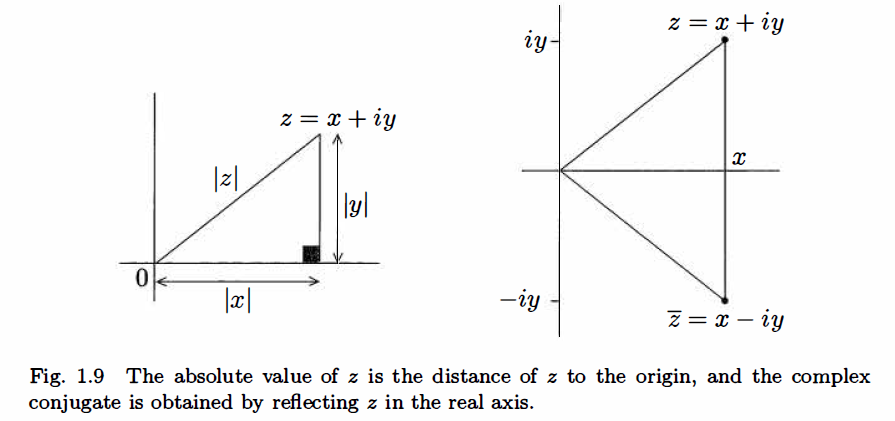
\includegraphics[width=0.7\textwidth]{./SaltChapter/fig-1-9}
\end{center}
\caption{복소수의 절대값은 원점에서의 거리이고, 켤레복소수는 실수축에 대칭인 복소수이다.}
\label{fig-1-9}
\end{figure}

\begin{salt_exercise} \label{ex-1-14}
직표좌표로 $z_1, z_2$를 써서 $|z_1z_2| = |z_1|\cdot |z_2|$임을 확인하라.
\end{salt_exercise}

복소수 $z=x+iy$ ($x,y\in\mathbb R$)의 켤레복소수 $\bar z$는
$$
\bar z = x - iy
$$
로 정의한다.
복소평면에서 $\bar z$는 $z$를 실수축으로 대칭시켜 얻는다.
그림 \ref{fig-1-9}의 오른쪽을 참고하라.
기하학적 표현으로부터 복소수 $z_1, z_2\in\mathbb C$에 대하여
다음이 성립함을 확인할 수 있다.
$$
\overline{z_1+z_2} = \overline{z_1} + \overline{z_2},
\quad
\overline{z_1\cdot z_2} = \overline{z_1} \cdot \overline{z_2}.
$$

다음 성질도 쉽게 얻을 수 있다.
$$
\bar{\bar z} = z, \quad z\bar z  = |z|^2 \quad
\Re(z) = \frac{z+\bar z}2, \quad \Im(z) = \frac{z-\bar z}{2i}.
$$

\begin{salt_exercise} \label{ex-1-15}
위의 등식 4개를 증명하라.
\end{salt_exercise}

\begin{salt_exercise} \label{ex-1-16}
모든 복소수 $z\in\mathbb C$에 대하여
$|z|=|\bar z|$, $|\Re(z)|\le |z|$, $|\Im(z)| \le z$임을 증명하고
각각에 대하여 기하학적으로 설명하라.
\end{salt_exercise}

\begin{salt_exercise} \label{ex-1-17}
$|a|<1$과 $|z|\le 1$을 만족하는 $a,z\in\mathbb C$에 대하여
$\left| \dfrac{z-a}{1-\bar a z}\right| \le 1$을 보여라.
\end{salt_exercise}

\begin{salt_exercise} \label{ex-1-18}
계수가 $c_0, c_1, \ldots, c_d\in\mathbb R$이고 $c_d\ne0$인 다항식
$p(z) = c_0+c_1z+\cdots + c_dz^d$을 생각하자.
$w\in\mathbb C$가 $p(w)=0$을 만족하면 $p(\bar w)=0$도 성립함을 보여라.
\end{salt_exercise}

\begin{salt_exercise} \label{ex-1-19}
복소수 $0, a, b \in\mathbb C$가 만드는 삼각형의 면적은
$\left| \dfrac{\Im(a\bar b)}2\right|$임을 보여라.
\end{salt_exercise}

\begin{salt_exercise} \label{ex-1-20}
임의의 복소수 $z_1,z_2, z_3$에 대하여
$i\det \begin{pmatrix}
1 & z_1 & \overline{z_1} \\
1 & z_2 & \overline{z_2} \\
1 & z_3 & \overline{z_3} 
\end{pmatrix}$는 실수임을 증명하라.
\end{salt_exercise}

\begin{salt_exercise} \label{ex-1-21}
임의의 두 복소수 $z_1, z_2$가
$|z_1+z_2|^2 + |z_1-z_2|^2 =2(|z_1|^2+|z_2|^2)$을 만족함을 보여라.
이 등식의 기하학적 의미는 무엇인가?
\end{salt_exercise}

\section{$\mathbb C$의 위상}








